% This document provides the style to be used for a MSc Thesis at the
% Parallel and Distributed Systems group
\documentclass[11pt,twoside,a4paper,openright]{report}

% use babel for proper hyphenation
\usepackage[british]{babel}
% Graphics: like the DUT logo on the front cover
\usepackage[dvips]{graphicx}
%Enables [H] for figures.
\usepackage{float}
% FONT: times
\usepackage{times}
% for url's use "\url{http://www.google.com/}"
\usepackage{url}
% To allow margin adjustments
\usepackage{changepage}
% To allow listings.
\usepackage{listings}
% To inserts to do's
\usepackage{todonotes}
% Boxed verbatim for experiments
\usepackage{fancyvrb}
% Side by side packages
\usepackage{subfigure}
% bib in order of appearance
\bibliographystyle{ieeetr}

\newsavebox{\FVerbBox}
\newenvironment{FVerbatim}
 {\VerbatimEnvironment
  \begin{center}
  \begin{lrbox}{\FVerbBox}
  \begin{BVerbatim}}
 {\end{BVerbatim}
  \end{lrbox}
  \fbox{\usebox{\FVerbBox}}
  \end{center}}

\begin{document}

%%%%%%%%%%%%%%%%%%%%%%%%%%%%%%%%%%%%%%%%%%%%%%%%%%%%%%%%%%%%%%%%%%%%%%%%%%%%%%%
\hoffset=1.63cm
\oddsidemargin=0in
\evensidemargin=0in
\textwidth=5in

%%%%%%%%%%%%%%%%%%%%%%%%%%%%%%%%%%%%%%%%%%%%%%%%%%%%%%%%%%%%%%%%%%%%%%%%%%%%%%%
\parindent=1em

\pagestyle{empty}

% FRONTCOVER
\begin{titlepage}

\null\vfill

\begin{center}
\LARGE{Software Performance Engineering in Complex Distributed Systems}
\end{center}

\vspace{1.5cm}

\begin{center}
Laurens F. D. Versluis\\
L.F.D.Versluis@student.tudelft.nl
\end{center}

\vfill

\centering
\begin{figure}[!b]
\captionsetup[subfigure]{labelformat=empty}
\begin{subfigure}{0.4\textwidth}
\centering

\includegraphics[height=3cm]{pics/triblerlogo}
\caption{}
\end{subfigure}%
\begin{subfigure}{0.6\textwidth}
\centering
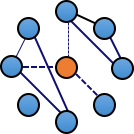
\includegraphics[height=3cm]{pics/dslogo}
\caption{}
\end{subfigure}%
\end{figure}

\begin{figure}[!b]
\centering

\includegraphics[height=2cm]{pics/TUDLogo}
\end{figure}


\vspace{2.0cm}

\end{titlepage}


% EMPTY PAGE
\cleardoublepage

\pagestyle{plain}

% TITLE PAGE: page i (hidden)
\begin{titlepage}

  \begin{center}
  \null\vfill
    \begin{center}
    \LARGE{Software Performance Engineering in Complex Distributed Systems}
    \end{center}

    \vspace{3cm}

    \begin{large}
    Master's Thesis in Computer Science
    \end{large}

    \vspace{1.5cm}

    \begin{normalsize}
	Distributed Systems group\\
    Faculty of Electrical Engineering, Mathematics, and Computer Science\\
    Delft University of Technology
    \end{normalsize}

    \vspace{2.0cm}

    \begin{normalsize}
    Laurens F. D. Versluis
    \end{normalsize}

    \vspace{1.0cm}

    % <MM> DD, YYYY
    \today

  \vfill
  \end{center}

\end{titlepage}



% GRADUATION DATA AND ABSTRACT: pages ii and iii (hidden)
%De aankondiging bevat de spreker, titel, plaats, datum en tijd, samenstelling van de afstudeercommissie en een korte samenvatting (maximaal 25 regels).
\thispagestyle{empty}

\noindent \textbf{Author}\\
\begin{tabular}{l}
Laurens F. D. Versluis\\
\\
\end{tabular}\\
\noindent \textbf{Title}\\
\begin{tabular}{l}
Addressing database constrained self organizing \& distributed systems\\
\\
\end{tabular}\\
\noindent \textbf{MSc presentation}\\
\begin{tabular}{l}
% <MM> DD, YYYY (like \today)
Dijkstrazaal, HB09.150\\
EEMCS, Delft\\
15:00-16:00, August 29, 2016
\\
\end{tabular}

\vspace{1.1cm}

\noindent \textbf{Graduation Committee}\\
\begin{tabular}{ll}
% The order of listing the names: Graduation prof, supervisor(s), others ordered by title + alphabetical
%examples:
%prof. dr. ir. H. J. Sips (chair) & Delft University of Technology \\
%ir. dr. D. H. J. Epema           & Delft University of Technology \\
dr. ir. J. A. Pouwelse            & Delft University of Technology \\
dr. ir. M. Zuniga                 & Delft University of Technology \\
dr. ir. A. Bozzon                 & Delft University of Technology \\

\end{tabular}

\begin{abstract} %de abstract bevat alleen een korte samenvatting van de inhoud van het onderzoek
TBD.



\end{abstract}

% \clearpage



\pagenumbering{roman}
\setcounter{page}{4}

% EMPTY PAGE: page iv
\cleardoublepage

% OPTIONAL QUOTATION: page v
%\pagestyle{empty}

\null\vfill

\begin{center}
\emph{``TODO QUOTE''} -- TODO QUOTED PERSON
\end{center}

\vspace{10cm}

\clearpage


% EMPTY PAGE: page vi
%\cleardoublepage

% PREFACE: page v
\chapter*{Preface}
\addcontentsline{toc}{chapter}{Preface}
The increasing surveillance by governments who seek to get a hold on the Internet is showing its presence more and more.
In countries such as China and X, where censorship is common practice shows that there is an (increasing) need for anonymity online.

To combat this practice, Tribler ....

Anonymous downloading....

People want youtube-like experience, fast and anonymous difficult. Tribler aims for this.

TBD.

\vspace{1\baselineskip}

\noindent
Acknowledges go here.

\vspace{1\baselineskip}

\noindent
Laurens Freydis Dene Versluis

\vspace{1\baselineskip}

\noindent
Delft, The Netherlands

\noindent
\today

% EMPTY PAGE: page vi
\cleardoublepage

% TABLE OF CONTENTS: starting at page vii
\setcounter{tocdepth}{1}
\tableofcontents

\cleardoublepage

\pagenumbering{arabic}
\setcounter{page}{1}

% CHAPTERS ... For instance: History/Prior Work, Design/Implementation, Experiments
% INTRODUCTION
\chapter{Introduction}
\label{chp:introduction}
Tribler is a peer-to-peer BitTorrent client that attempts to fully decentralize downloading, uploading and streaming of content.

Tribler focusses on the goals:
\begin{itemize}
    \item Allow for secure and private communication and sharing of data.
    \item Enforce user contribution in the network
    \item Make it impossible to shut Tribler down, unless the Internet itself as a whole gets taken down.
\end{itemize}

A fully decentralized ecosystem i.e. no central components present, is Tribler's approach to achieve these goals.
Tribler has been designed and build with this focus~\cite{Pouwelse-tribler,Bakker-tribler}.
A distributed network requires both the presence and collaboration of participants, called peers, to be able to achieve this.

This thesis was conducted to improve the connectability and overall performance of Tribler, by identifying and removing bottlenecks present in the system.

\begin{figure}
	\centerline{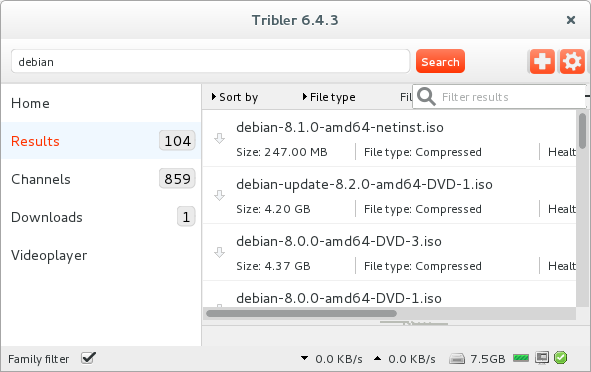
\includegraphics[scale=0.6]{introduction/figs/tribler-screenshot.png}}
	\caption{Screenshot of Tribler v6.4.3.}
	\label{fig:tribler-screenshot}
\end{figure}

\section{BitTorrent protocol}
When sharing files by using the BitTorrent protocol, a peer that uploads parts of a file to another peer, is called a seeder.
A peer that is downloading a file of a seeder is called a leecher.
Any peer can be both a seeder and leecher at the same time, and join the network at any given time.

The ratio between the total data downloaded and uploaded is called the seeding ratio \cite{Cohen-bittorrent}.
The seeding ratio can be seen as an indication of the level of collaboration i.e. giving back resources to the network.

Seeding can be seen as an interaction between peers, where the seeder aids the leeching peer.
By utilizing the seeders upload bandwith, the leeching peer can use his download bandwidth to download a file.
While there is a clear incentive for the leecher by downloading the desired file, there is none for the seeder.
Especially since the leecher has a little chance of becoming also be a seeder for the original seeder \cite{Lai-Incentives}.

Having peers actively and persistently contribute to the network will increase the network's health which in turn provides several benefits for all peers.
A more healthy network results in a higher availability of seeders and results in high download speeds.
It has been shown that private communities where the seeding ratio is high, provides better download conditions \cite{meulpolder-privatecommunities}.
In these private communities, trackers i.e. central components introduce peers to each other using the Tit-for-tat approach \cite{cohen-titfortat}.
The Tit-for-Tat approach is aiding peers who have aided you in the past,
The absence of trackers, which is often the case in public networks, results in free-riding \cite{Adar-Freeriding}.
A free-riding peer does not or gives little back to the network while receiving all benefits i.e. download without any restriction.
BitTorrent applies a variation of the Tit-for-tat strategy, optimistic chocking, to combat this problem.
The Tit-for-Tat strategy is to only provide help to peers that return this help.
% TODO explain the optimistic chocking approach
However, it has been shown that this approach is not effective in battling abuse \cite{Pouwelse-tribler}.

\section{Tribler}
Tribler wants to achieve a high global seeding ratio by making it beneficial to have such a ratio.
Nodes can award each other with higher cooperation if a node has a reputation of being cooperative,
while malicious nodes are prevented from tampering and freeriding.
Within Tribler anonymous connections have been implemented recently using onion routing~\cite{Plak-anonymous,ruigrok-anonymous,tanaskoski-anonymous}.
This feature allows downloaders to become indistinguishable from other users in the network save guarding their privacy.
Every data packet has to be forwarded
by a number of intermediate hops between the downloader and seeder~\cite{Plak-anonymous,tanaskoski-anonymous}.
The total cost of bandwidth per file is increased,
because it has to be forwarded by multiple nodes.
but also the number of nodes helping a single node downloading a file increases.
The increase in nodes working together increases the necessity of an incentive system to reward collaboration.

Dispersy is middleware for data dissemination in a network.
Dispersy is used heavily within Tribler and is maintained by the Tribler organisation.
Our work is build upon Dispersy.
Dispersy is used to exchange data between two specific nodes~\cite{zeilemaker-dispersy}.
Functionality was added to Dispersy during the thesis.
The additions are described in chapter \ref{chapt:design}.

\section{Document structure}
Chapter \ref{chp:introduction} provides information on Tribler.
Chapter \ref{chp:problem-description} presents an overview of some of the problems Tribler is currently facing.

%Problem description
\chapter{Problem description}
\label{chp:problem-description}

Tribler's goal is to offer a YouTube-like experience with similar performance and ease of use.
All Tribler's features are implemented in a completely decentralized manner, not relying on any centralized component.

Numerous initiatives exist around these goals of re-decentralisation and performance.
However, none of them gathered any significant usage compared to the social media usage levels. 
For instance, YouTube features one billion unique monthly users \cite{mainka2014government} and there are 1.8 billion monthly active Facebook users \cite{sharma2016strategies}.

The problem is that the performance, usability, and features offered by decentralised alternatives are inferior when compared to the experience offered by central solutions.
Creating academically pure self-organising systems such as Tribler has proven to be notoriously difficult.
For example, the extensive list of 194 projects which all aim to create an alternative Internet experience using decentralisations shows the amount of years spent and lines of code produced \cite{redecentralize2016alternative}.
Most of these projects are abandoned and few of them have actual real-world usage.

\begin{figure}[!h]
	\makebox[\textwidth][c]{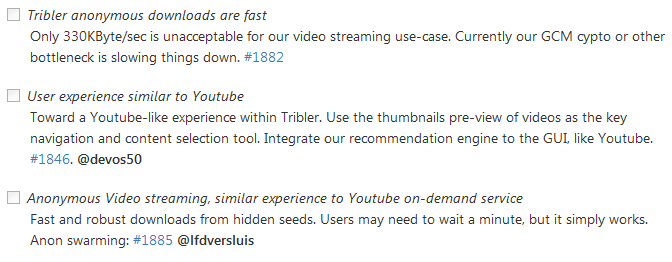
\includegraphics[width=\linewidth]{problemDescription/images/roadmap}}
	\caption{Three of the six uncompleted Tribler roadmap items.}
	\label{fig:tribler_roadmap}
\end{figure}

The Tribler project created a roadmap -- available on its GitHub repository -- to offer the same service, features, user experience, and performance as the YouTube video-on-demand service.
However, especially the poor performance of Tribler is hampering wide-spread adoption and usage. Figure~\ref{fig:tribler_roadmap} shows three of the six main uncompleted roadmap items.

\section{Key performance optimizations}

Tribler can be seen as a large and complex distributed system.
Metrics from OpenHUB show that Tribler, along with its components, features more than 169 thousand lines of code, received contributions from 111 unique contributors and took approximately 44 years of effort \cite{openhub2016tribler}.

In large and complex systems there are likely to be many performance issue present, often referred to as \emph{bottlenecks}.
J. M. Juran's Pareto principle admonishes that one should "Concentrate on the vital few, not the trivial many" \cite{ammons2004finding}. This principle is also known as the 80/20 rule.
Concretely, this means that resolving the vital bottlenecks yields the best diminishing returns, even for large systems such as Tribler.
After careful scrutiny it was decided that the most vital bottleneck to address, within the context of a nine month thesis, is Tribler's database I/O.

\section{Addressing blocking I/O}
\label{sct:triblers_database_dependency}

The problem we address within this thesis is the underlying reason for poor performance and unacceptable user experience. 
Measurements dating back from 2013 indicate that Tribler's performance is I/O-bound \cite{pouwelse2014reduce}.
Especially with slow hard disks, but also with fast SSD storage the main performance bottleneck seems to be around database access.
With our focus on the fundamental issue we believe we can make a significant step forward in making decentralized technology able to compete with centralized solutions on large-scale usage.

\begin{figure}[!h]
	\makebox[\textwidth][c]{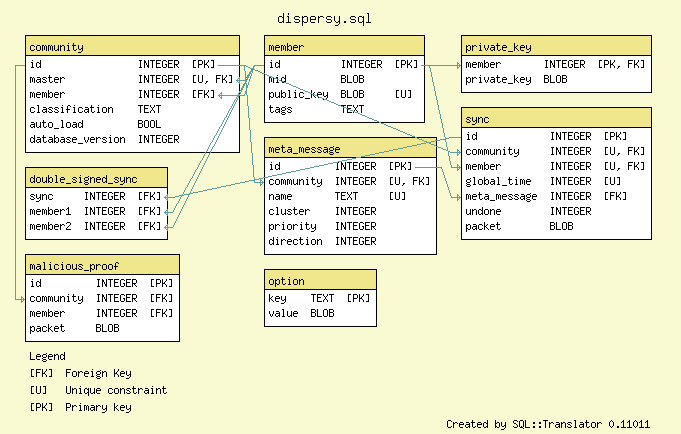
\includegraphics[width=\linewidth]{problemDescription/images/dispersy_database_schema}}
	\caption{The database schema of Dispersy, (source: Johan Pouwelse, 2013) \cite{pouwelse2013documentation}.}
	\label{fig:dispersy_database_schema}
\end{figure}

All information within Tribler is stored in a database for persistence and ease of use.
Information about the network i.e. peers, messages and authentication is stored in a separate database managed by the Distributed Permission System (Dispersy).
Dispersy is an elastic database system written in the Python programming language and uses SQLite as its underlying database engine.
It lies at the heart of Tribler, providing the means to discover peers and content in a decentralized way while offering security and anonymity.

Dispersy is fully decentralized with the exception of bootstrap servers.
It can run on systems with a large number of nodes, without any sever architecture needed \cite{dispersy2016dispersy, zeilemaker2013dispersy}.
All nodes perform the same algorithmic procedures and tasks and do not differentiate between any node i.e. all nodes are equal.

Furthermore, Dispersy provides on-to-one and one-to-many data dissemination mechanisms to forward data to nodes.
Eventually, all data will reach all nodes in the network, overcoming challenging network conditions.
The current overview of the database structure is presented in Figure~\ref{fig:dispersy_database_schema} (Johan Pouwelse, 2013).

These databases are becoming a key performance bottleneck \cite{pouwelse2014reduce}.
Back in May 2013 measurements indicated that Tribler read and wrote 660 Megabytes per hour to and from disk.
The next measurement in April 2014 showed this number was somewhat reduced to 623.
In May 2014 efforts were made to reduce this enormous amount of I/O; by batching database statements the number dropped to 538 Megabytes per hour.

So far this metric has only been measured sporadically by hand, running Tribler for an arbitrarily amount of time and check the amount of I/O by using htop\footnote{\url{http://hisham.hm/htop/}}.
htop produces an overview similar to Figure \ref{fig:iotop_tribler_april_2014} (Johan Pouwelse, 2014).
Measurements to observe to which extent Dispersy is responsible for these numbers were never conducted, however it is strongly suspected by the Tribler developers that Dispersy is responsible for most of it.
Since 2014 no work or measurements have been done related to this issue.

\begin{figure}[!h]
	\makebox[\textwidth][c]{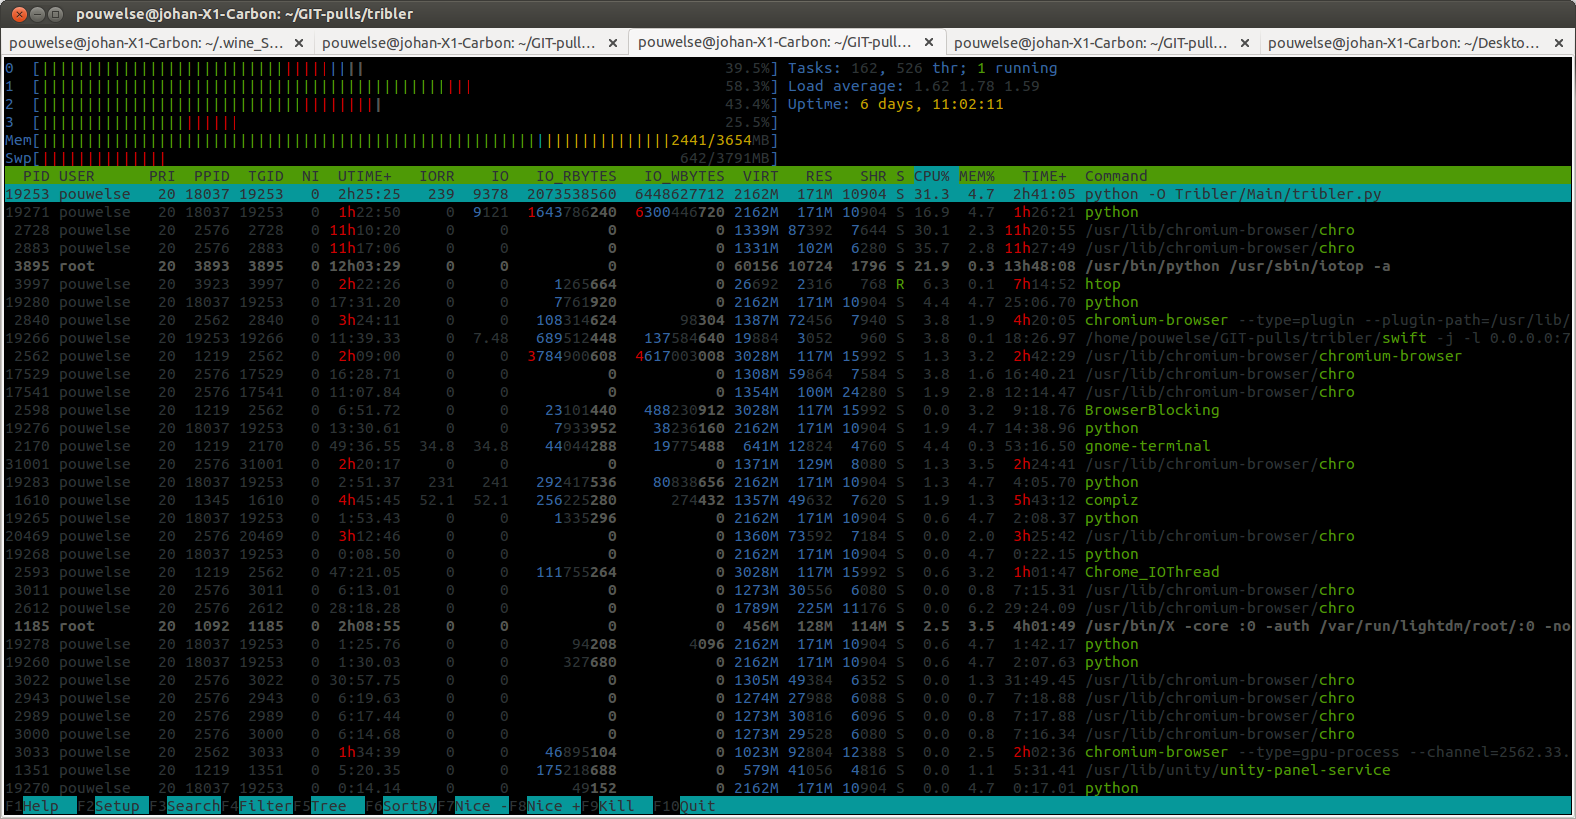
\includegraphics[width=0.9\paperwidth]{iointribler/images/iotop}}
	\caption{A screenshot of htop showing Tribler's I/O, (source: Johan Pouwelse, 2014 \cite{pouwelse2014reduce}).}
	\label{fig:iotop_tribler_april_2014}
\end{figure}

\subsection{Blocking I/O}
One of the main causes of Tribler's dramatic performance can be explained by the blocking behaviour of I/O.
Currently, Dispersy is deeply embedded into Tribler, running on the same (main) thread Tribler is running on.
Tribler, just like Dispersy, is written in the Python programming language.
In Python, a thread performing an I/O operation will block, causing all operations on the thread to suspend.
This means whenever Tribler or Dispersy performs I/O all functions of Tribler and Dispersy halt.
With the enormous amount of I/O Tribler is performing, this forms a huge limiting factor on the responsiveness and therefore performance of Tribler.

When a thread suspends, other threads can take over and perform operations, yet besides the main thread there are only two additional threads in Tribler: the Graphical User Interface (GUI) thread and the Dispersy endpoint thread.
As the name implies, the GUI is running on the GUI thread as the framework Tribler currently uses requires this.
Ironically, the Dispersy endpoint thread was introduced because of the blocking I/O behaviour.
Under heavy load, Dispersy drops packets because it cannot keep up.
Processing packets is done on the main thread and as this thread frequently blocks, the buffers overflow causing packet loss.
These two threads do not saturate the available processing time offered by the main thread blocking, leading to wasting valuable CPU cycles.

Furthermore, Tribler has seen several changes to its code base including the addition of the MultiChain: Tribler's own Blockchain-like structure \cite{norberhuis2015multichain}.
This feature heavily relies on its database to store blocks and other information about the user and other peers.
Moreover, the MultiChain makes use of its own database rather than Dispersy's.
Norberhuis points out: \enquote{The information is stored in two places within Tribler and this could be eliminated. It would reduce the disk footprint and the amount of read/write transactions as only one database would have to be maintained. The I/O ineractions are a problem according to Tribler maintainers.} \cite{norberhuis2015multichain}, yet numbers on how much I/O the MultiChain generates are not presented.
This makes it hard to estimate Tribler's current I/O rates.

Furthermore, a feature called \enquote{credit mining} is currently in development that will also interact with the database of Tribler.
There are no metrics on the current situation of Tribler and it's hard if not impossible to estimate the impact of any addition to come.
Currently, there is a lack of insight in these metrics, or a lack of \emph{software performance engineering}, causing the exact extent of the problem to be unknown.

%\section{Asynchronous I/O}
%\label{sec:async-programming}

\section{A lack of software performance engineering}

\begin{figure}[!h]
	\makebox[\textwidth][c]{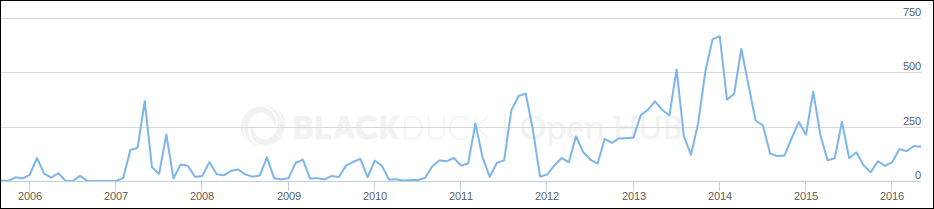
\includegraphics[width=\linewidth]{problemDescription/images/commits_openhub.png}}
	\caption{The distribution of commits on Tribler (source: OpenHUB, 2016 \cite{openhub2016tribler}).}
	\label{fig:commits_openhub}
\end{figure}

Nowadays, programs are evolving at a rapid speed and Tribler is no exception. 
Since 2005 Tribler is under continuous development, over seventeen thousands commits have been made, spanning more than a decade \cite{openhub2016tribler}.
The distribution of these commits can be seen in Figure~\ref{fig:commits_openhub}.
Code commits to fix bugs, refactor code, enhance or add functionality are pushed to code repositories at a frequent rate.
It is important that software performance engineering is a part of this process: performance should not get compromised by changes, if any it should improve.
Naturally trade-offs can be made performance wise, but it should be done with a clear understanding of the consequences.

For the past three years, attempts have been made to monitor the performance, yet with little success.
The first attempt was to create probes using Systemtap\footnote{\url{https://sourceware.org/systemtap/}}.
System tap is a tool for \enquote{instrumenting the Linux kernel for analyzing performance and functional problems}, (Jacob et al. 2008) \cite{jacob2008systemtap}.
While some success was reported, this system is no longer being maintained nor functional.
After this, code was added to the Dispersy code base to track and log if a function was running longer than a fixed amount of time.
While this implementation does provide some insight, its workings are crude and only covering some of the functions present.
For instance, it cannot handle asynchronous constructions.
Tribler did not have any observation system integrated, leaving the development team in the dark regarding its performance.

It is apparent that there is a lack of software performance engineering in the development cycle of Tribler.
Performance has never been one of the priorities in Tribler's lifetime; only 6\% of all tickets on GitHub are (indirectly) related to performance.
To ensure performance will no longer degrade realistic benchmarks need to be developed which Tribler can be tested with.
Changes can then be compared against the current codebase, tracking important performance statistics such as the amount of I/O, run time of functions, throughput and responsiveness.
These benchmarks can then be integrated into a regression testing system which can be integrated in our Jenkins continuous integration system.
Using Jenkins, performance regression tests can run on every proposed change and at predetermined moments, having a continuous updated overview of Tribler's performance metrics.

% https://github.com/Tribler/tribler/issues/15
% https://github.com/Tribler/tribler/issues/77
% experiment framework: https://github.com/Tribler/tribler/issues/114
% latency grpahs? https://github.com/Tribler/tribler/issues/119
% speed of streaming: https://github.com/Tribler/tribler/issues/134
% of course: https://github.com/Tribler/tribler/issues/3
% nightly runs: https://github.com/Tribler/tribler/issues/184
% extreme cpu ticket: https://github.com/Tribler/tribler/issues/197
% slow startup time ticket: https://github.com/Tribler/tribler/issues/255

\section{Realistic benchmarks}
Directly related to the performance problem is the benchmark problem.
In order to improve user performance we require making assumptions about realistic use cases.
Each user has different usage patterns, hardware and network conditions, all affecting performance.
Creating one of more several benchmarks testing several scenario's is required to accurately tune the system for real world usage.
At the same time, a benchmark cannot consume too much time.
Benchmarking is by nature time consuming \cite{huang2014performance}, however running long regression tests per commit done on a pull request will severely strain the development speed.

Therefore, it is important to create a reference benchmark which has a close resemblance to real world usage without consuming too much time.

The next step is to introduce a solution, tracking changes in vital numbers such as CPU consumption or I/O produced.
Any improvement indicated by this benchmark should reflect improvement for real world users.
This system should benchmark the current code base against proposed changes, capturing any differences in performance.


%\section{OLD TEXT}
%Only by comparing different builds can one gain insight into performance changes.
%Currently Tribler lacks this insight.
%As Tribler is heavy I/O-based and likely I/O-bound, it is crucial to have these numbers.
%A breakdown of database statements is needed and the amount of I/O that is generated.
%Recently a block-chain like structure called the Multi-Chain was added to Tribler and soon another feature called credit mining will be introduced as well.
%The impact and increase of I/O caused by these additions are unknown.

%Ideally, we would like to run regression tests on multiple platforms powered by our Jenkins continuous integration system as visualized by Figure X \todo{make figure.}.
%This regression test will feature average use cases and automatic graph generation to give developers an instant overview of their changes.
%This system has to run automatically whenever a pull request is opened on GitHub.
%Efforts can then be made to optimize the I/O output and improve the performance of Tribler.

%\section{Resolving bottlenecks}
%To improve the performance of Tribler, (I/O) bottlenecks to need to be removed.
%The key problem here is how to identify and resolve bottlenecks in a complex system such as Tribler.

%By careful inspection of the usage of I/O, we identified that Tribler's I/O is blocking the main thread.
%Many programming languages have support for parallelization, allowing multiple functions to be executed at the same time by using threads.
%Tribler does not have access to this paradigm as it's written in the Python programming language.
%Python lacks this feature as only one thread can run in the Python interpreter at any time because of the Global Interpreter Lock (GIL).
%However, a thread does release the GIL when it's performing a blocking I/O operation, allowing other threads to get a hold of the GIL and run.
%Leveraging this trait to gain performance is a huge step forward towards solving the (I/O) bottleneck Tribler is currently facing.

%\section{Tribler's code base}
%At the same time, Tribler's current code base has a severe lack of (unit) tests, structure and documentation and contains dead code.
%The current version has been in development for over nine months, is plagued with bugs and non-functioning on some platforms.
%As of writing, the code is only tested on a single Unix operating system.
%Tribler, however, is available for all three major operating systems: Windows, Mac OS and Unix distributions.
%As users are reporting platform specific bugs, it is evidently important that automated testing on all three platforms are realized.
%All this results in long and complex debugging processes and creates a steep learning curve for new students joining the project and might withhold members of the open-source community to start contributing.

%While it's not this thesis primary goal, refactoring the code involved with the bottlenecks and properly documenting and testing %this refactored code is a secondary goal of this thesis, aiding in lowering the learning curve and improving the stability of %the Tribler code base.

% \section{Connectability}
% One of the problems Tribler faces is the connectability of its users.
% Users can be behind e.g. firewalls that prevent incoming or outgoing connections.
% Currently, Tribler employs NAT and Firewall Traversal [CITE], yet the success of this method is limited.
%The Tribler team has implemented their own Distributed Hash Table (DHT) in python while existing libraries such as LibTorrent also offer these.
% These implementations should be tested to see if changing to a library offers a significant boost in terms of exchange or speed.

%When users are downloading anonymously, they are inside so-called `hidden swarms'.
%These hidden swarms are not present in e.g. LibTorrent's DHT and therefore information from peers has to be exchanged between peers themselves by means of introducing peers to each other (PEX).
%By making use of Dispersy, Tribler creates rendezvous points to introduce peers to each other.
%If these rendezvous points are not connectible, PEX cannot take place.
%Solving this may be done by always connecting to the same port (chosen by the user or a default) and ask the user to forward that port.
%If users are not willing to do so, they can be penalized.
%This penalty can be for example not able to download anonymously at all, receive half the amount of credits when credit mining (see [CITE]) or limited download speed.

% \section{Anonymous download speed}
% To allow for anonymous downloading, Tribler uses a Tor-like technique to create so called `anon tunnels'.
% To increase download speed and prevent a bottleneck in the network hampering the overall download speed, several tunnels are built to download simultaneously from [CITE?].
% Since this Tor-like technique includes cryptographic functions, having multiple tunnels running concurrently results in a lot of cryptographic calls being executed.
% Stok et al. profiled Tribler using a gumby\footnote{Gumby is Tribler's experiment running framework.} experiment. This experiment showed that a lot of processing time is spent on encrypting and decrypting packets [CITE] as well as serializing and deserializing data.
% Currently, the CPU power is a bottleneck when downloading using the anonymous tunnels.
% By offloading the encryption and decryption of packets to a separate core, the workload on the core on which Tribler is running can be reduced.
% This should yield an increased download speed and better spread of workload overall as more packets can be processed per time unit.

% \section{Package serialization}
% One of the core components of Tribler is Dispersy. 
% Dispersy is a fully decentralized elastic database capable of communicating packets and exchanging peers.
% Both Dispersy and Tribler make use of python' built-in serialization function.
% The profile ran by Stok et al. [CITE] indicated that a significant amount of CPU resources is spent on serializing data when sending or receiving UDP packets.
% As previously explained, running multiple threads at once does not result in code being executed concurrently.
% Cap'n Proto is a serialization framework that offloads the serialization of packets to a C++ process, which bypasses the global interpreter lock.
% This means that the other threads -- who are still affected by the global interpreter lock -- can immediately continue their work as the locks is released once the offloading to the C++ code base is done.

% \section{Responsiveness}
% Since Tribler is written in the python language, calls on any thread will cause other threads to halt their execution. % this is wrong.
% Normally two separate threads can run code in parallel as they generally do not touch each other's state.
% The cause of this is the Global Interpreter Lock (GIL) which states that only one function can be executed at a time.
% In its current state, the Graphical User Interface (GUI) of Tribler will block if it's doing some CPU or I/O intensive work.
% This yields a scenario in which the user is unable to perform any action, which is not user friendly.
% In some cases the operating system itself will show e.g. a warning or visualisation that the process is not responding.
% To solve this issue, heavy operations should be done on separate threads or processes which are not monitored by the GIL.
% Several libraries that are written in C/C++ are a good example of this.
% Once the code of such a library is invoked and the execution is offloaded to the C/C++ code, the GIl is released, allowing other python code to ran in parallel.
% Another approach is using the python framework Twisted.
% Twisted has implemented a thread pool that also bypasses this GIL.
% By rewriting CPU or I/O intensive code to make use of this thread pool in an asynchronous way, the responsiveness of Tribler can be improved.

% \section{Code quality and testing}
% Tribler's current code base is in a bare state.
% The current version that has been in development for over nine months now is plagued with bugs and is non-functioning.
% Furthermore, there is a severe lack of unit tests, a lot of the code is undocumented and unnecessary complex and structure and flow are missing.
% This results in long and complex debugging processes when bugs are found and raise the bar for new contributors to get familiar with the code base.

% As of writing, the code is only tested on a single Unix operating system.
% Tribler, however, is available for all three major operating systems: Windows, Mac OS and Unix distributions.
% As users are reporting platform specific bugs, it is evidently important that automated testing on all three platforms are realized.

% Refactoring the code is necessary in order to regain the structure and lower the code complexity.
% Furthermore, proper unit tests are required to ensure Tribler's stability now and in the future.
% These tests have to be executed on build machines that run different operating systems, preferably with various configurations e.g. 32 and 64 bit architectures or different library versions.

\section{Objective and research questions}
\label{chp2:sct:objectives-research-questions}
The objective of this thesis is to improve the performance and responsiveness of Tribler and to introduce a regression test system.
The verification of the performance regression test system is done by focussing on removing Tribler's biggest bottleneck present: blocking database I/O.
By resolving this bottleneck, important metrics tracked by this regression test system should show positive changes, indicating improvement.
%In general, projects facing similar issues can adopt the practices applied when changes made to the Tribler code base.\\

The research presented in this thesis was carried out in cooperation with the Tribler team. 
The Tribler team consists of both staff members of the Technical University of Delft as well as Bachelor and Master students.
Based on the objectives of Tribler, this thesis aims to answer the main research question formulated below.\\

\textbf{Main Research Question:} How can we improve Tribler's performance, responsiveness and throughput?\\

To answer this main research question, we have defined three research questions below. Each of these research questions will be justified as why they contribute to the main research question.\\

\textbf{Research Question 1:} Can a system such as Tribler benefit from asynchrony?\\

To improve performance and responsiveness, parts of Tribler can be rewritten to become asynchronous.
By performing tasks asynchronously the performance and responsiveness of a program can improve.
However, an asynchronous approach can have its drawbacks. 
One of these drawbacks is that it requires a different mindset for the programmers as the whole call chain and structure of a program becomes different.
Identifying these drawbacks and deciding if the benefits outweigh the costs is necessary to prevent the current state from worsening. \\

\noindent
\textbf{Research Question 2:} How do we incorporate software performance engineering into Tribler to gain insight into performance statistics?\\

Currently, not a single developer has insight into how well Tribler performs and what impact changes have on Tribler in its current state.
To be able to conclude performance changes do not negatively impact the performance of Tribler, we can apply software performance engineering.
Software performance engineering focuses on introducing performance regression tests and benchmarks into the development cycle.
By making use of these regression tests, Tribler developers finally get insight into vital metrics which are desperately needed.\\

\textbf{Research Question 3:} How do we create benchmarks which are a representative use case of Tribler?\\

Ultimately, the end user should benefit from performance enhancements.
The key issue here is to define metrics and workloads to benchmark with.
Metrics need to properly capture changes to accurately measure the impact of any modification.
Additionally, if the workload does not represent a realistic use-case the benchmark may be flawed, rendering the outcome unreliable and inaccurate.

A second constraint is the run time of a benchmark.
Preferably, the regression testing system should not clog the throughput of the current test architecture.
Running an one hour benchmark per change per pull request will severely strain the development speed.

\section{Main contributions}
The main contributions of this thesis are as follows.
First, we elaborate on the subject of multitasking and parallelization in the context of the Python programming language and provide arguments where asynchronous programming is preferred over synchronous programming, using Tribler as a case study.
We then resolve the vital I/O bottleneck currently present in Tribler using asynchrony and a multi-threaded approach.
This is done by introducing the Storm database framework into Tribler and creating a database manager with an asynchronous, non-blocking yet serialized interface.
Next, we introduce software performance engineering into Tribler's development process by adding a regression testing system that benchmarks different versions of the same code base to gain insight into performance metrics such as disk I/O.
Finally, experimental results and measurements will be provided to confirm the main goal of this thesis i.e. improving responsiveness, performance and user experience.

%Related work
\chapter{Related work}

\section{Parallelism and asynchrony in Python}
\label{sct:parallelism_and_asynchrony_in_python}
Parallelize Python by removing the GIL, introducing asynchronous behaviour or by other means is a topic that regularly returns in e.g. the Python mailing list, topics as PyCon and other events \cite{python2015global}.
To gain performance, many attempts have been made to alter Python or remove the GIL to fully benefit from multiple CPU's.
To date, no one has ever succeeded in removing the GIL and meet the (hard) requirements for replacement \cite{python2015global}.

On of the most well-known alternative implementations of Python is PyPy.
It makes use of a tracing Just-in-Time compiler to produce optimized code \cite{bolz2009tracing}.
By doing so, PyPy offers increased speed, reduced memory usage and support for stackless mode while providing a highly compatibility with existing python code \cite{pypy2016pypy}.
PyPy's geometric average is 7.6 times faster than CPython (normal Python) \cite{pypy2016speed}.
While it has many popular libraries ported to be used with Pypy, it still lacks some common used packages.
Moreover, most of these libraries are not available on the official packaging repositories of Ubuntu and/or Debian.

Two other popular implementations are JPython and IronPython.
Both of these projects have removed the GIL and can fully exploit multiprocessor systems \cite{python2015global}.

JPython is a Python interpreter implemented in Java. It can be integrated in Java applications and allows python applications to be compiled into Java classes.
Using JPython, Python after compiled to java bytecode will run in the Jython virtual machine, giving full access to all Java APIs and classes \cite{jython2016why}.

IronPython does basically the same as JPython, compiling the source to in-memory bytecode and runs it on the Dynamic Language Runtime \cite{ironpython2014}.
It allows developers to run Python using the .NET framework.

To illustrate the attempts to remove the GIL are still on going, Larry Hastings presented ``The Gilectomy'' at PyCon 2016.
He showed that removing the GIL is fairly easy, but has a huge negative impact on CPython's performance.
Additionally, he explained the reason why this performance loss was observed and names some methods that may make ``The Gilectomy'' a viable alternative to CPython.\\

Libraries and frameworks that introduce asynchrony are also available in large numbers.
In particular, many projects exist that attempt to make I/O asynchronous \cite{asyncio2016python}.

Twisted is an event-driven networking engine written in Python.
It allows for event-driven and asynchronous programming using deferreds.
Twisted has a custom event-loop called the reactor, on which tasks can be scheduled.
This reactor handles callbacks/errbacks fired by deferreds and contains many utility functions and classes to perform asynchronous and non-blocking calls.
Unlike many libraries and frameworks available, Twisted is available on the official repositories of Ubuntu and Debian and is a well tested, mature framework.

In 2012 Guido van Rossum embarked on a journey to add asynchronous I/O to the Python 3 standard library.
The asyncore library is showing it's age and according van Rossum \enquote{We have to throw it away and forget it ever existed.} (Guido van Rossum, PyCon 2013).
Van Rossum wrote a new Python Enhancement Proposal (PEP)\footnote{https://www.python.org/dev/peps/pep-3156/} and implemented a new framework \enquote{Tulip} \cite{edge2013pycon}.
Tulip's implementation and features are inspired by many well-known asynchronous frameworks such as Twisted and Tornado.
Tulip features Coroutines, Futures and Tasks.
Coroutines are equivalent to callbacks which are python generators under the hood.
Futures are similar to deferreds in Twisted, which is a placeholder for a value that is currently being computed.
Tasks are Futures wrapped in Coroutines.
Just like Twisted, Tulip features an event loop which multiplexes different activities such as callbacks and signals. 
It was added to Python 3.3 and is now part of the Python standard library in Python 3.4.
There are no plans to make Tulip available for older Python versions such as 2.7 or 3.2.

Decorated Concurrency (DECO) uses the multiprocessing package of Python to parallelize functions using a ``concurrent'' decorator \cite{sherman2016deco}.
Different processes have their own GIL, which allows for parallel processing.
Similarly, the ``synchronized''  inserts synchronization events to automatically refactors assignments of the results of ``concurrent'' function calls to happen during synchronization events.
However, because of the overhead of creating a new process and communicating between different processes, this approach is only viable for heavy loads that generally can run on its own and requires heavy computation.

\section{Regression testing}
Regression testing has been extensively studied both in research as industrial appliances.
\todo{Add related work regarding regression testing.}

\section{Profilers}
Resolving bottlenecks using profilers has been applied for many years: \cite{pesterev2010locating, gorelick2014high, fan2013performance}.
By default, Python ships three profilers:

\begin{enumerate}
	\item cProfile is a C extension that has reasonable overhead. It is the current recommended profiler. It provides the same interface as the ``profiler'' profiler.
	\item profiler is a profiler written in pure Python. It adds a lot of overhead and its usage is discouraged. However, because it's written in Python, it does allow for easier extension than it's C counterpart cProfile.
	\item hotshot was an experimental C module which is now deprecated as its no longer maintained. While it's still present, the module may be dropped in a future version of Python.
\end{enumerate}

Alternatively, profilers have been developed by the open-source community.
Yappi is a profiler written in the C language that is thread-aware, allowing automatic profiling of multi-threaded applications [CITE]\todo{cite}.
It provides options to measure CPU or wall time, sort the output by various parameters and support the callgrind and pstat output formats.

Savrun-Yeni{\c{c}}eri et al. introduced an event-based profiler that performs better than the Python standard profilers which requires modest implementation effort \cite{savrun2015efficient}.
Their profiler helps users find bottlenecks in programs, aids language implementers to improve the performance of their language implementation and allows the comparison and evaluation of different languages using cross-language benchmarks.\\

%Experimentation
\chapter{Experimental results}
\label{cpt:experiments}

\begin{table}[h]
	\centering
	\caption{Specifications of the setup used during the idle iotop measurement of Tribler 6.6.0-pre-exp.}
	\label{table:virtual_machine_specs}
	\begin{tabular}{l|l}
		\textbf{Component} 	& \textbf{Specifications} \\ \hline
		OS   				& Ubuntu 15.10 \\
		Python version		& 2.7.10 \\
		CPU					& 1 Core with 4 processors (2.5 GHz each) \\ 
		HDD					& 25 GB  \\ 
		RAM					& 8 GB  \\
	\end{tabular}
\end{table}

To evaluate Tribler's current situation and to validate our implementations are working correctly, experiments have been conducted.
In this chapter we elaborate on these experiments and discuss the results. 
All experiments with the exception of one have been conduction on a virtual private server whose specifications can be found in Table\ref{table:virtual_machine_specs}.

\section{Tribler's I/O over the years}
As explained in Section~\ref{sct:triblers_database_dependency}, Tribler's I/O has been a problem for years.
To observe if and how the amount of I/O has changed over time, we have performed measurements on four \todo{change if needed} different versions of Tribler using iotop\footnote{\url{http://guichaz.free.fr/iotop/}}.
The versions and their release dates are depicted in Table~\ref{table:tribler_version_dates}.

As these measurements were never performed systematically, it is vital to perform these measurement now to observe if any changes have occurred between releases and document them.
This will provide valuable insight in Tribler's behaviour and the extent of the problem.
Moreover it will show us if the amount of I/O is being reduced since the creating of the ticker on GitHub.

\begin{table}[h]
	\centering
	\caption{The versions of Tribler and their release dates.}
	\label{table:tribler_version_dates}
	\begin{tabular}{|l|l|}
		\hline
		Tribler version & Release date \\ \hline
		6.3.5           & 2014-11-06   \\ \hline
		6.4.3           & 2015-01-21   \\ \hline
		6.5.2           & 2016-05-13   \\ \hline
		6.6.0-exp1      & 2016-07-26   \\ \hline
	\end{tabular}
\end{table}

\begin{figure}[!h]
	\centering
	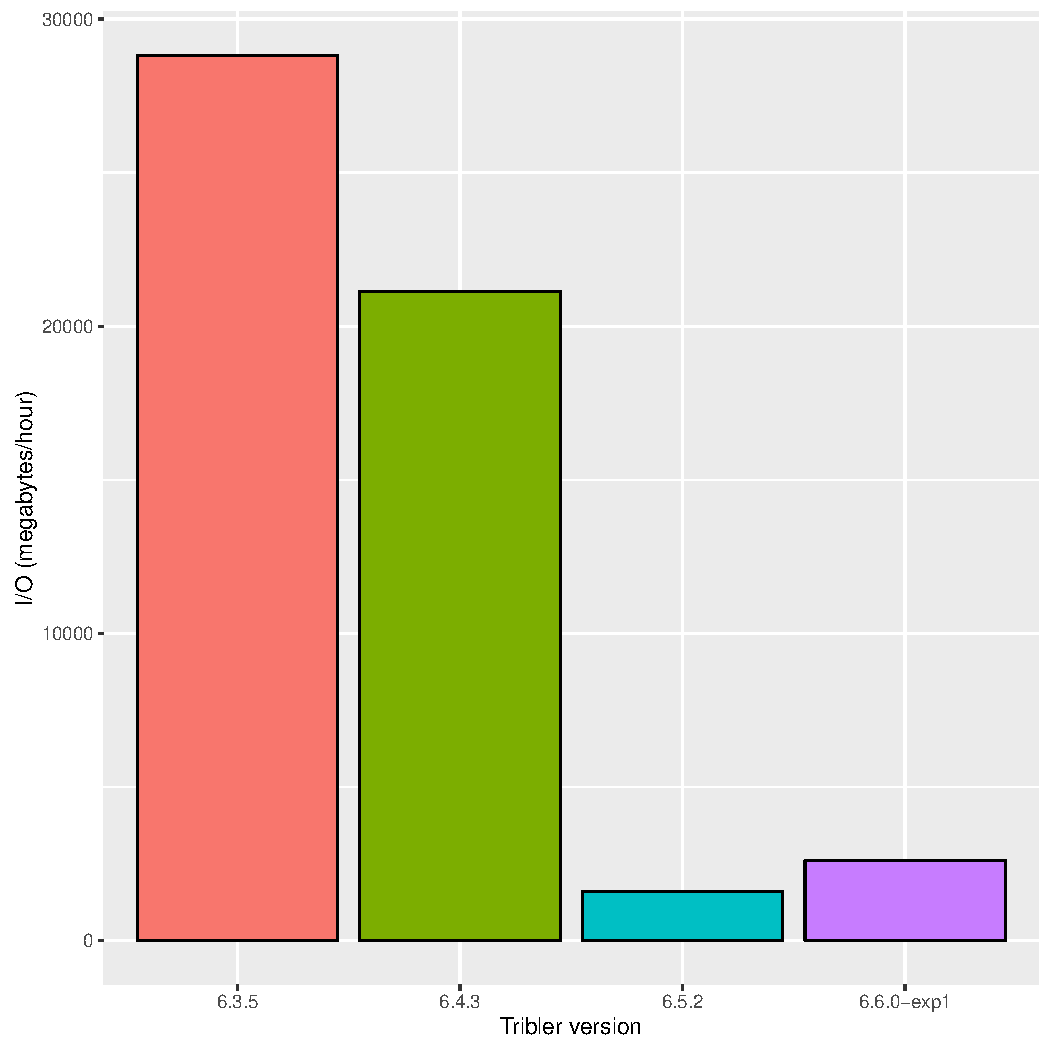
\includegraphics[width=\linewidth]{experimentation/images/io_history}
	\caption{The amount of I/O per version of Tribler.}
	\label{fig:io_history}
\end{figure} 

Each version of Tribler will run for one hour idle, using a clean state directory i.e. no prior knowledge of the network and its contents.
During the idle run, Tribler will start discovering peers and content such as channels and torrents, storing the obtained data in the database which gets flushed to disk.
Additionally, peers will start requesting data from this Tribler instance such as search and peer exchange requests, causing Tribler to read data from the database.
These read and writes operations will be monitored by iotop and the amounts automatically accumulated.
After one hour, the amount of read and write I/O is noted down and Tribler is shutdown.

The results of this experiment are visible in Figure~\ref{fig:io_history}.
From this figure we observe that Tribler's I/O has been reduced significantly in version 6.5.2.
This decrease was the result of batching multiple database queries and periodically flush them to disk, an effective optimization technique also applied in other work \cite{ouyang2011beyond, lin2009database}. 
Furthermore we observe the amount of I/O is increasing again in the latest 6.6.0-exp1 release due to the MultiChain feature added. 

Peculiarly, the numbers observed in this experiment are significantly higher than the numbers reported in the original ticket.
We believe the reason two reasons contribute to these numbers.
The first one is due to the 100 mbit connection of the experiment machine, providing excellent connectability conditions. 
Secondly, the fact that this instance began with a clean state directory while running idle, provides ideal conditions for Tribler to spend most of its resources on discovering peers and content.

\begin{table}[]
	\centering
	\caption{The packets collected for each version by Tribler when running idle for one hour using a clean state directory.}
	\label{table:packets_collected_idle}
	\begin{tabular}{|l|l|l|}
		\hline
		Paket type                         & Tribler version & Amount  \\ \hline
		\multirow{4}{*}{Dispersy-identity} & 6.3.5           & 20,026  \\ \cline{2-3} 
		& 6.4.3           & 38,268  \\ \cline{2-3} 
		& 6.5.2           & 46,890  \\ \cline{2-3} 
		& 6.6.0-exp1      & 41,480  \\ \hline
		\multirow{4}{*}{Dispersy-undo-own} & 6.3.5           & 40,594  \\ \cline{2-3} 
		& 6.4.3           & 45,095  \\ \cline{2-3} 
		& 6.5.2           & 47,409  \\ \cline{2-3} 
		& 6.6.0-exp1      & 44,279  \\ \hline
		\multirow{4}{*}{votecast}          & 6.3.5           & 44,990  \\ \cline{2-3} 
		& 6.4.3           & 90,339  \\ \cline{2-3} 
		& 6.5.2           & 116,557 \\ \cline{2-3} 
		& 6.6.0-exp1      & 96,509  \\ \hline
	\end{tabular}
\end{table}

To observe the cost versus the benefits, we have tracked the amount of packets Tribler managed to synchronize while running one hour idle using a clean state directory for each version.
The results are visible in Table~\ref{table:packets_collected_idle}.
From this table we conclude that while version 6.3.5 and 6.4.3 perform much more I/O, the amount of packets obtained is significantly less.
From these numbers we this conclude that the cost of having high I/O rates is not justified by the benefits as they perform even worse. 
Interestingly, the numbers of the latest 6.6.0-exp1 version are similar to that of 6.4.3, while we cannot explain this fully, we believe it may be caused by external network conditions or the MultiChain feature.

In conclusion, we believe that the I/O rate of Tribler does not show a correlation with the amount of packets synchronized. As the I/O rate of Tribler rises again in the latest version, possibly because of the MultiChain feature requiring additional computations, it shows the urgency of the I/O to become asynchronous and non-blocking.

\section{I/O breakdown}

\begin{table}[h]
	\centering
	\caption{Specifications of the setup used during the idle iotop measurement of Tribler 6.6.0-pre-exp.}
	\label{table:tribler_idle}
	\begin{tabular}{l|l}
		\hline
		\textbf{Packet type}	& \textbf{Amount} \\ \hline
		Operating System   	& Ubuntu 16.04 LTS \\
		Python version		& 2.7.12 \\
		CPU					& Intel Core i5-2410M \\ 
		HDD					& Samsung 850 EVO 250GB  \\ 
		RAM					& 8 GB DDR3 1600MHz \\
	\end{tabular}
\end{table}

\begin{table}[]
	\centering
	\caption{A breakdown of the Dispersy database function calls when running Tribler idle for one hour using a clean state directory.}
	\label{table:breakdown_tribler_idle}
	\begin{tabular}{|l|r|r|l|l|l|}
		\hline
		\textbf{Query}	& \textbf{Amount of calls} & \textbf{Total time (s)} & \textbf{Max}  & \textbf{Average} & \textbf{Min} \\ \hline
		execute			& 1,099,211	& 36.068 	& 0.24959	& 0.00003	& 0.00001 \\ \hline
		commit			& 65	& 11.089	& 1.12432	& 0.17061	& 0.00001 \\ \hline
		executemany		& 4282	& 0.233  	& 0.00071	& 0.00005	& 0.00001 \\ \hline
	\end{tabular}
\end{table}

To observe the individual components separately, we have created a breakdown of the database queries performed by Dispersy. \todo{Run this experiment on the ubuntu 15.10 machine.}

\section{Tribler's performance}

To measure the performance gain of Tribler, we have conducted two sets of experiments where two instances of Tribler, one with a synchronous, blocking Dispersy implementation and one with the asynchronous, non-blocking version of Dispersy, are compared.

In the first experiment we have ran Tribler idle for one hour while querying the Twisted event loop every 100 milliseconds for delayed calls.
By doing so we can observe if certain tasks have been delayed past their set time of execution i.e. measure the latency in the system.

In the second experiment we have stress-tested Tribler's new API.
By requesting data from an endpoint at several rates per second, we can observe the throughput, response times, variance in these response times and throughput of Tribler.

\subsection{Measuring the latency of Tribler}

\begin{figure}[!h]
	\centering
	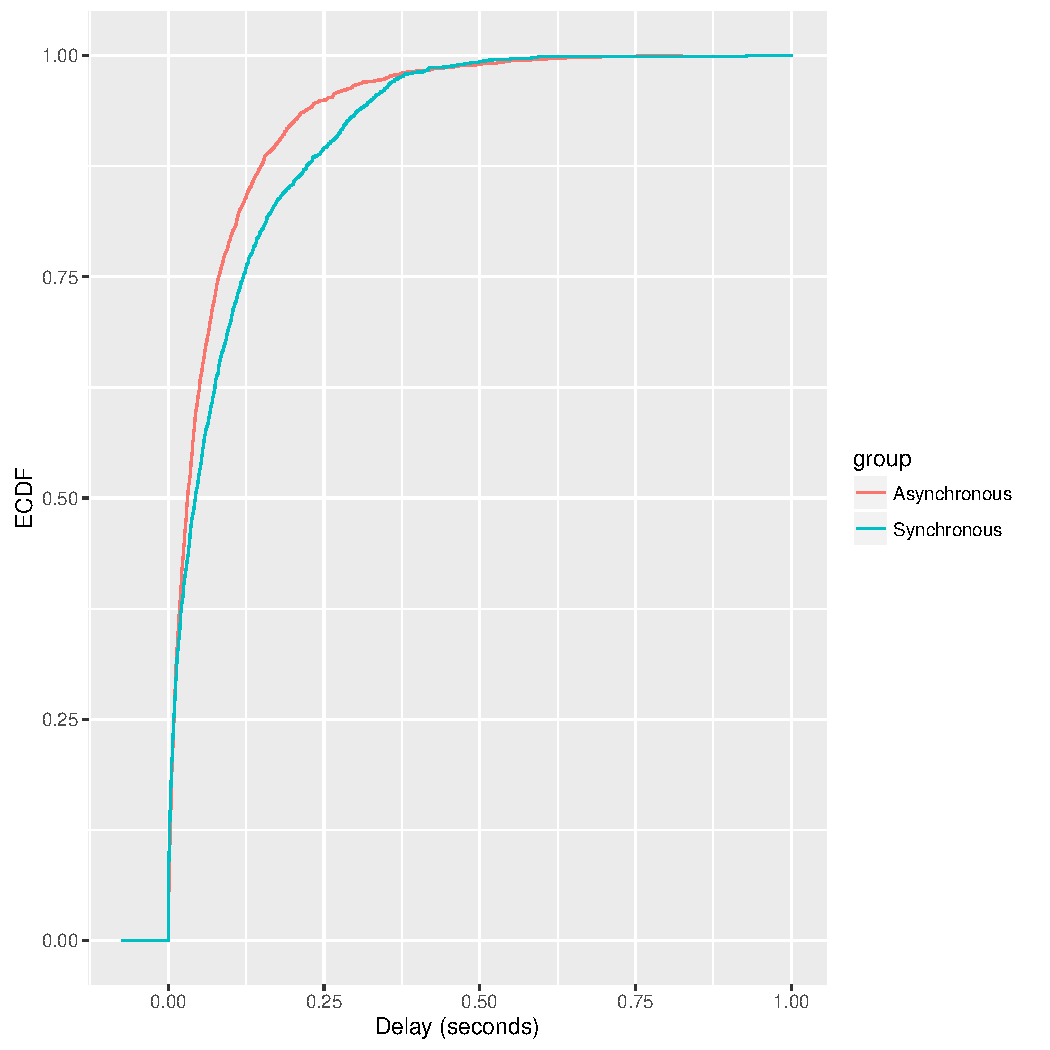
\includegraphics[width=\linewidth]{experimentation/images/ecdf_latency_idle}
	\caption{An ECDF plot of the latency when running Tribler idle.}
	\label{fig:ecdf_latency_idle}
\end{figure} 

In this experiment we have compared two versions of Tribler, one with Dispersy having blocking, synchronous I/O and one with Dispersy running StormDBManager and thus having non-blocking, asynchronous I/O.
Each instance of Tribler was run one hour idle where every 100 milliseconds the event loop of Twisted was queried for delayed calls.
By observing if scheduled calls are past their set time of execution, we can measure the amount of delay or \emph{latency} in the system.
Latency occurs when the twisted reactor thread is blocked or busy with a task that takes a relative long time to complete, causing other tasks to become delayed.
Latency is therefore directly related to the responsiveness of a program.
The lower the latency, the more responsive a system is.

In theory, making functions asynchronous slices them into smaller \enquote{chunks} which can be executed interleaved, creating a more responsive system as e.g. user actions will be executed in between (background) operations.

In this experiment the hypothesis is that the latency of the asynchronous version will be lower than its synchronous counterpart.
Since Tribler is running idle it has more resources i.e. CPU time available to tend to Dispersy which is running in the background, which most likely will cause the difference to be smaller than when Tribler is experiencing additional load.
However, we believe the average may still be significant enough to prefer the asynchronous implementation.

After running the experiment, we have created an empirical cumulative distribution function (ECDF) plot of the delayed calls, visible in Figure~\ref{fig:ecdf_latency_idle}.
From this figure we observe that the asynchronous version performs better than the synchronous version.
On average, the synchronous version has a latency of 87 milliseconds, where the asynchronous version has a latency of 66 milliseconds, a difference of 24\%.
Furthermore, the synchronous case has more outliers, some even touching the one second mark.
This observations are enough to confirm the hypothesis: both on average and in maxima the latency of the asynchronous version are lower.

\subsection{Measuring the responsiveness of Tribler}

To measure the responsiveness of Tribler while under load, we have stress tested the API of Tribler using the procedure described in Section~\ref{ssct:benchmark_3}.

In this experiment we use a state directory containing around 1200 channels.
By querying Tribler's channel API endpoint for all discovered channels, all channels in the database will be fetched and returned.
As this is Tribler's heaviest endpoint in terms of computation, it's the best way to put Tribler under load.
In total the experiment will be run six times, querying the channel endpoint exactly 1000 times per run using 1, 2, 5, 10, 15 and 20 requests per second respectively.
By tracking the response times, the amount of requests per seconds and the throughput the API can offer, we can measure the gain in responsiveness and thus in performance (T) of Tribler.
We expect that the asynchronous version will outperform the synchronous version significantly in both response times as throughput.

\begin{table}[!h]
	\centering
	\caption{The results of the six experiments runs with and without asynchronous, non-blocking I/O in Dispersy.}
	\label{table:responsiveness_tribler_load}
	\begin{tabular}{|c|c|c|c|c|c|c|c|}
		\hline
		Req./s              & Async. & Avg (ms) & Min & Max & Std. Dev. & T (KB/s) & Resp./s \\ \hline
		\multirow{2}{*}{1}  & \xmark      & 315 & 53  & 4774 & 615.90    & 564.19            & 0.9         \\ \cline{2-8} 
		& \cmark      & 134 & 57  & 2576 & 189.89    & 612.60            & 1.0         \\ \hline
		\multirow{2}{*}{2}  & \xmark       & 237 & 52  & 4524 & 475.31    & 1049.31           & 1.7         \\ \cline{2-8} 
		& \cmark      & 113 & 56  & 1224 & 162.62    & 1197.90           & 1.9         \\ \hline
		\multirow{2}{*}{5}  & \xmark       & 143 & 52  & 2865 & 259.64    & 2399.57           & 3.9         \\ \cline{2-8} 
		& \cmark      & 67  & 56  & 846  & 38.50     & 3058.27           & 5.0         \\ \hline
		\multirow{2}{*}{10} & \xmark       & 135 & 54  & 3338 & 259.37    & 3827.02           & 6.2         \\ \cline{2-8} 
		& \cmark      & 89  & 52  & 1138 & 92.58     & 5435.71           & 8.8         \\ \hline
		\multirow{2}{*}{15} & \xmark       & 133 & 51  & 4678 & 382.57    & 4521.46           & 7.3         \\ \cline{2-8} 
		& \cmark      & 88  & 52  & 963  & 82.23     & 6799.35           & 11.0        \\ \hline
		\multirow{2}{*}{20} & \xmark       & 109 & 51  & 3400 & 239.23    & 5599.75           & 9.1         \\ \cline{2-8} 
		& \cmark      & 74  & 52  & 1051 & 57.37     & 8264.01           & 13.4        \\ \hline
	\end{tabular}
\end{table}

\begin{figure}[!h]
	\centering
	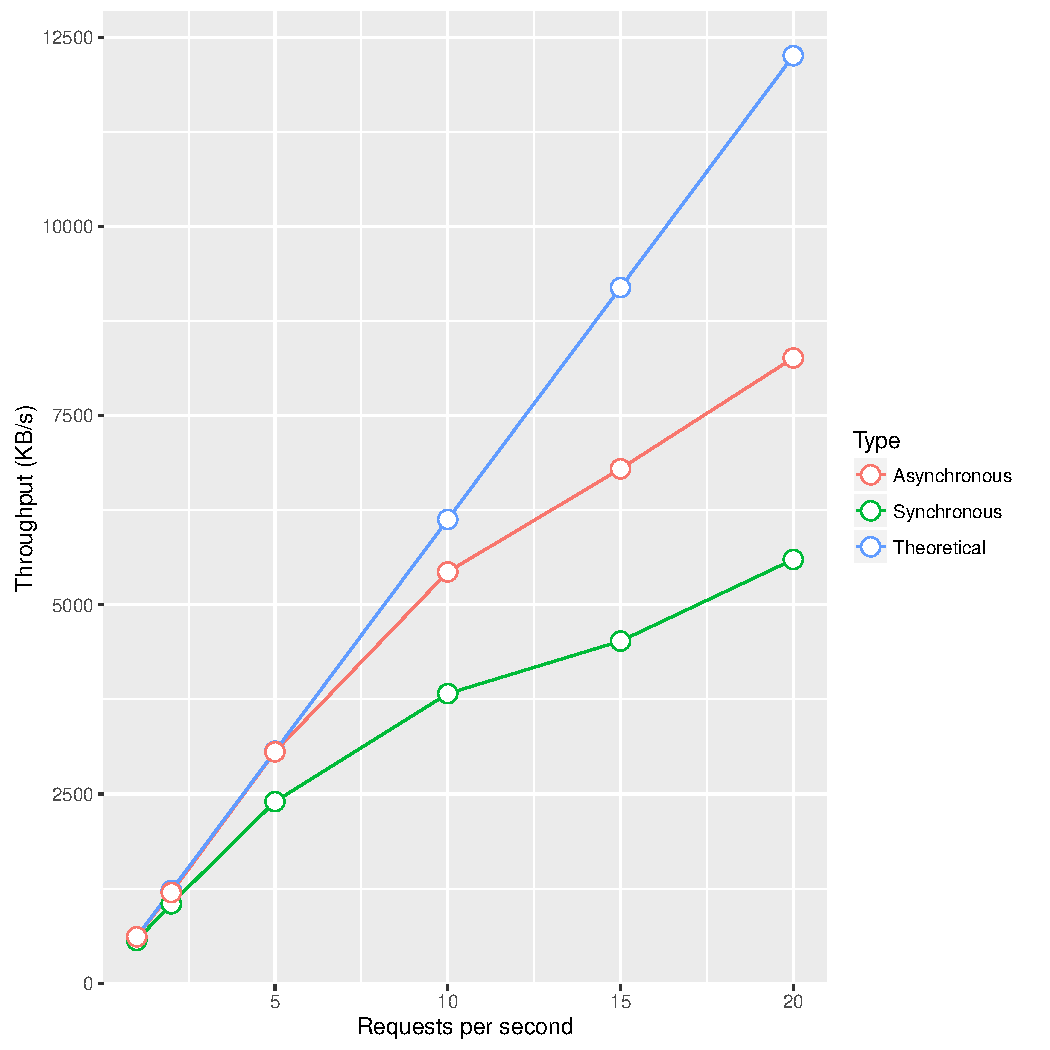
\includegraphics[width=\linewidth]{experimentation/images/throughput_requests.pdf}
	\caption{The throughput theoretically and of Tribler running Dispersy with asynchronous, non-blocking and synchronous, blocking I/O }
	\label{fig:throughput_requests}
\end{figure} 

The results of the experiment can be found in Table~\ref{table:responsiveness_tribler_load}.
From this table we observe that asynchronous version has a significant less amount of response time, both on average and in maximal duration.
The reduction in response times (on average) ranges between 32.1\% and 57.5\%.
As the responsiveness of a program can be directly linked to its performance (see Section~\ref{ssct:benchmark_3}), this looks very promising.
Interesting to note here is that the average response times of the synchronous version go down when the amount of requests per second goes up.
We believe this may be due to Twisted caching responses.

Another indication that the system has become more responsive is the the standard deviation.
For every run the standard deviation of the asynchronous version is significantly less than its synchronous counterpart, indicating the response times are more stable than the synchronous version. 
This can be explained by the slicing of tasks because of asynchrony; as tasks are more interleaved, smaller tasks such as a request will be processed in between bigger tasks, yielding a higher and more stable responsivity.

A third promising statistic is the throughput.
As the response is 613 kilobytes (KB) in size, the theoretical maximum throughput will be 613, 1226, 3065, 6130, 9195 and 12260 KB/s, respectively.
If we plot the theoretical, asynchronous and the synchronous throughput we obtain Figure~\ref{fig:throughput_requests}.
As we can see the throughput of the asynchronous case lies close to the theoretical maximum until around the ten requests per second.
At this point Tribler starts to show signs of being overloaded, which is also visible in the table when looking at the amount of responses received per second.

At ten requests per second both the asynchronous and the synchronous version cannot keep up.
If we look at the responses per second for fifteen and twenty requests per second, we observe that the gap between requests and responses grows percentage wise.
The question that arises here is why Tribler can't provide 13.4 responses per second with fifteen requests per second as in the case with twenty.
Again we believe the answer lies in the Twisted framework.

As more tasks are scheduled on the event loop of Twisted, it will process each of them fairly where priority is given to the most delayed task.
Since there are now more requests pending, it will spend more computation power on the requests.
Even though this means that more responses per second can be provided, percentage wise the amount of replies per request drops: for fifteen requests this percentage is 73\% where for twenty requests per second this percentage is 67\%.

All in all, this experiment demonstrates that the asynchronous system has superior performance over the synchronous case, increasing the throughput up to 150\%.

\subsection{Validating the performance regression test system}

\begin{figure}[!h]
	\centering
	\makebox[\textwidth][c]{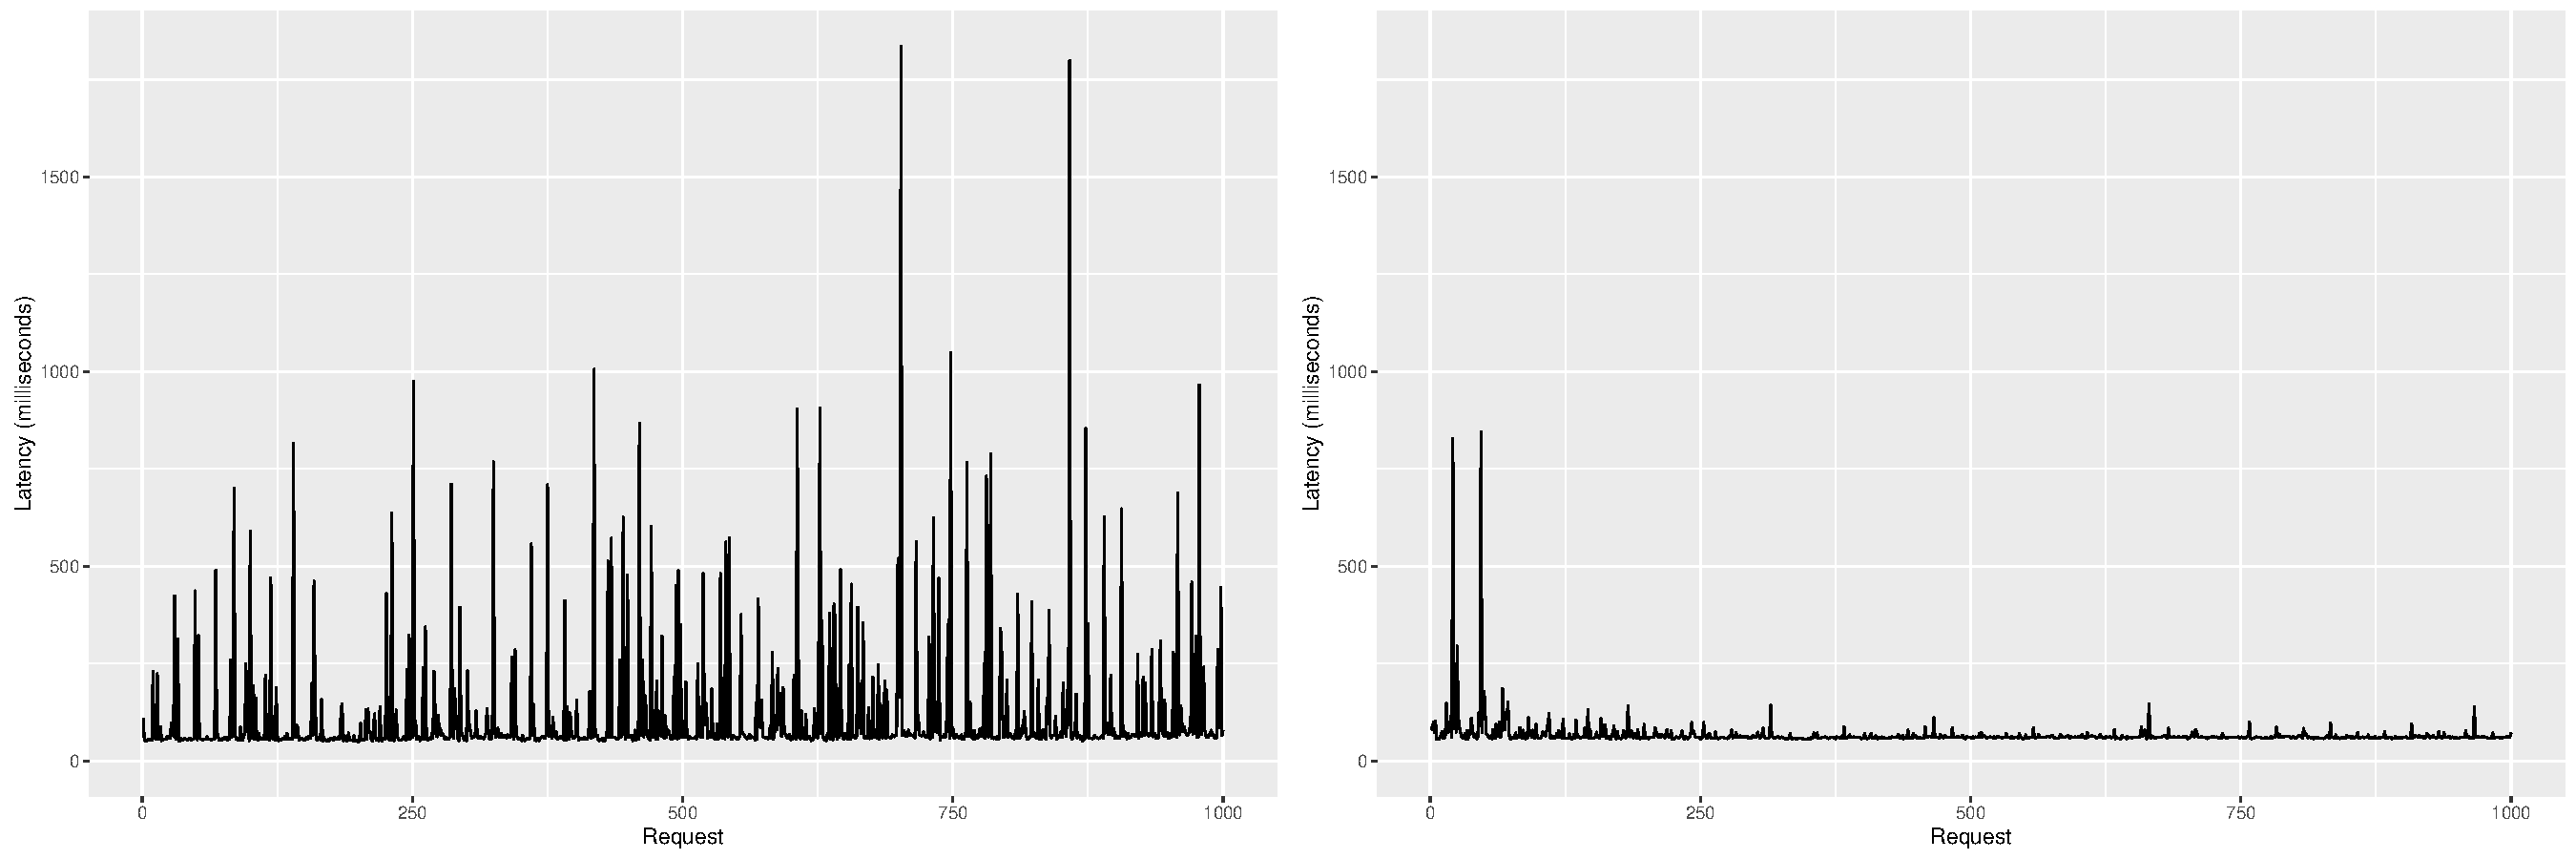
\includegraphics[width=0.9\paperwidth]{experimentation/images/response_times_comparison.pdf}}
	\caption{The comparison graph showing the response times of Tribler's API. Left: Tribler running Dispersy with synchronous, blocking I/O, right: Tribler running Dispersy with asynchronous, non-blocking I/O.}
	\label{fig:tribler_response_times_comparison}
\end{figure} 

To validate the performance regression system, we run the experiment above with 5 requests per second.
From the results, Gumby creates a side-by-side comparison graph and a table with an overview of the differences in the data obtained.

Figure~\ref{fig:tribler_response_times_comparison} shows the comparison graph generated.
From this figure, it is clear that the left hand side -- showing the current code base -- has higher response times than the right side.
From this graph it is immediately clear that the proposed changes have a positive impact on the responsiveness of the API.

To look at the data generated by the benchmark in more detail, the generated table shown in Figure~ \todo{todo} provides a breakdown of the data.
This breakdown highlights the average, minimum, maximum and standard deviation in response times as well as the throughput obtained.

From these figures we conclude that the performance regression test system provides a suitable overview for developers to get a quick overview of the current state.
%Conclusion
\chapter{Conclusion and Future Work}
\label{cpt:conclusion_and_future_work}

This thesis aims to contribute to the goal of re-decentralisation of systems such as Tribler to become as performant and as accessible as centralized solutions such as YouTube.
We have addressed Tribler's blocking database I/O, its main performance bottleneck, by integrating the Storm database framework into a new database manager: \enquote{StormDBManager}.
StormDBManager features a complete asynchronous, non-blocking interface for database access while still maintaining a serialized query execution strategy.
Furthermore we have provided deep insight into Tribler's and Dispersy's database usage, pinpointing functions that could be reviewed for query optimization.
By making Dispersy's database I/O asynchronous and non-blocking, we have improved Tribler's API throughput by up to 150\%, reduced its response times by up to 57.5\% and moved its longtail latencies to the 99th percentile up from the 90th percentile.

Additionally, we have created a regression testing system and prepared it to be integrated in our Jenkins continuous integration system to adopt software performance engineering in the development cycle, further maturing the project.
We have verified both the regression testing system and the resolving of the bottlenecks by providing experimental results.
We believe that with this performance boost and software performance engineering focus, we have contributed to Tribler's further years of research and strengthened Tribler's chances on becoming a decentralized alternative for YouTube-like streaming.

While we believe we made a significant step forward in both performance and software performance engineering, there are items left for future work.

As different platforms and operating systems may influence the performance of a program, it is useful to run regression tests on all platforms Tribler supports.
Deploying the regression test system on all platforms will ensure no regression occurs on one of them.

To remove the \enquote{raw queries} from all code bases, an object-relational mapping approach can be applied.
This will reduce the complexity of the system as all data will be contained in objects which are generally easier to modify and read from.
This will require extensive refactoring of Tribler and Dispersy's code bases.

While we have managed to move the longtail latencies to the 99th percentile and reduce the size of these latencies, there is still room for improvement.
Removing them completely by buffering or other means can lead to further improvements which could be investigated.

To improve performance further, moving Tribler from Python2 to Python3 is another possibility.
As we have seen, the Global Interpreter Lock in Python 3.2 and onwards has been updated to handle I/O-bound threads better.

To increase the speed of processing database queries, it can be investigated if we can use SQLite's multi-threaded support to process more queries.
While SQLite developers themselves admit SQLite has minimal multithreaded support, it can still be investigated to what extent we can leverage its support.

Improving the quality of Dispersy's tests is another item that was mentioned in this thesis.
It was found that passing all tests in Dispersy does not provide any guarantees beyond a basic level of correctness.
Improving and adding tests is required to increase the stability, maintainability and correctness of Dispersy.

A final item that we would like to highlight as future work is running benchmarks in a closed environment, disconnected from the Internet.
When running Tribler and Dispersy, it will connect to the Internet which may influence performance metrics such as I/O rates and amount of packets obtained.
Creating a closed environment with local peers will ensure that only those peers can communicate to one another.
These peers can then be instrumented to behave in a predetermined manner.
This will increase both the reliability and accuracy of the measurements made.



% BIBLIOGRAPHY
%\bibliographystyle{bib/latex8}
\bibliography{bib/bibliography}

%\appendix

%\include{appendix_a}

\end{document}

